\section{Ускорение точек тела с неподвижной точкой}

Дифференцируя формулу Эйлера $\vec{v} = \crossprod{\vec{\omega}}{\vec{r}}$,
получаем
\begin{equation}
  \vec{w} = \dt[\vec{v}] = \crossprod{\dt[\vec{\omega}]}{\vec{r}}
    + \crossprod{\vec{\omega}}{\dt[\vec{r}]}.
\end{equation}

Производная по времени от вектора угловой скорости определяет вектор
\textit{углового ускорения}
\begin{equation}
  \vec{\varepsilon} = \dt[\vec{\omega}].
\end{equation}
По величине и направлению этот вектор совпадает со \textit{скоростью движения
конца вектора $\vec{\omega}$ угловой скорости по его годографу}.

Замечая, что
\begin{equation*}
  \dt[\vec{r}] = \vec{v} = \crossprod{\vec{\omega}}{\vec{r}},
\end{equation*}
получим
\begin{equation}
  \begin{aligned}
    \vec{w} &= \crossprod{\vec{\varepsilon}}{\vec{r}} +
      \crossprod{\vec{\omega}}{\vec{v}} \\
    &= \crossprod{\vec{\varepsilon}}{\vec{r}} +
      \crossprod{\vec{\omega}}{\paren{\crossprod{\vec{\omega}}{\vec{r}}}}.
  \end{aligned}
\end{equation}

\begin{figure}[H]
  \centering
  \resizebox{\linewidth}{!}{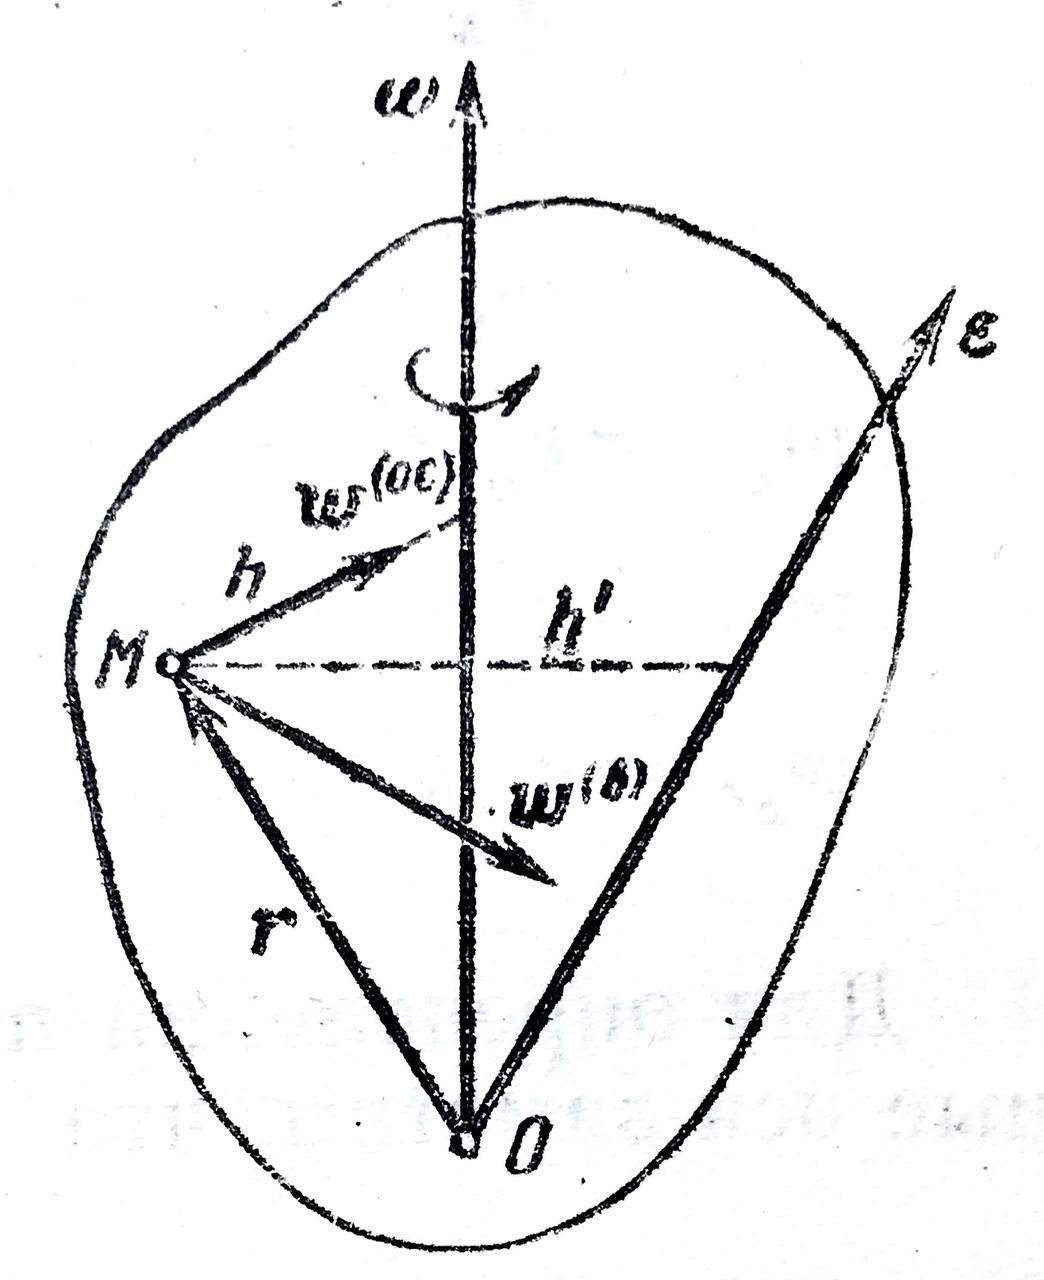
\includegraphics{src/mechanics/pictures/22_1.jpg}}

  \caption{}
  \label{fig:22_1}
\end{figure}

Первое слагаемое
\begin{equation}
  \vec{w}^\text{(в)} = \crossprod{\vec{\varepsilon}}{\vec{r}}
\end{equation}
представляет собой \textit{вращательное ускорение}; это --- вектор,
перпендикулярный к плоскости, проходящей через вектор углового ускорения и
вектор-радиус взятой точки тела. В отличие от случая вращения вокруг неподвижной
оси, вектор углового ускорения не лежит на той же прямой, что и вектор угловой
скорости, а направлен по некоторой прямой, проходящей через неподвижную точку;
эту прямую будем называть \textit{осью углового ускорения}.

Эта ось параллельна скорости конца вектора $\vec{\omega}$. Поэтому здесь вектор
вращательного ускорения перпендикулярен не радиусу вращения $h$, а отрезку $h'$,
представляющему собой кратчайшее расстояние от точки $M$ до оси углового
ускорения. По величине вращательное ускорение равно
\begin{equation}
  \label{eq:immovable_point:rotational_acceleration_length}
  w^\text{(в)} = \varepsilon h'.
\end{equation}

Второе слагаемое
\begin{equation*}
  \vec{w}^\text{(ос)} = \crossprod{\vec{\omega}}{\vec{v}} = 
    \crossprod{\vec{\omega}}{\paren{\crossprod{\vec{\omega}}{\vec{r}}}}
\end{equation*}
определяет \textit{осестремительное ускорение}. Оно направлено перпендикулярно к
плоскости, содержащей $\vec{\omega}$ и $\vec{v}$, то есть по кратчайшему
расстоянию между точкой $M$ и мгновенной осью, причём всегда в ту сторону,
откуда вращение $\vec{\omega}$ к $\vec{v}$ на наименьший угол видно
положительным. По величине осестремительное ускорение равно
\begin{equation}
  \label{eq:immovable_point:centripetal_acceleration_length}
  w^\text{(ос)} = \omega v \sin \frac{\pi}{2} = \omega \cdot \omega h
    = \omega^2 h.
\end{equation}

Таким образом, ускорение точек твёрдого тела, вращающегося вокруг неподвижного
центра, складывается геометрически из вращательной и осестремительной
составляющих.

\subsection{Список литературы}
\begin{enumerate}
  \item \cite{lourie}
\end{enumerate}

